\documentclass{article}

\usepackage{arxiv}
\usepackage[utf8]{inputenc} % allow utf-8 input
\usepackage[T1]{fontenc}    % use 8-bit T1 fonts
\usepackage{hyperref}       % hyperlinks
\usepackage{url}            % simple URL typesetting
\usepackage{booktabs}       % professional-quality tables
\usepackage{amsfonts}       % blackboard math symbols
\usepackage{nicefrac}       % compact symbols for 1/2, etc.
\usepackage{microtype}      % microtypography
\usepackage{cleveref}       % smart cross-referencing
\usepackage{lipsum}         % Can be removed after putting your text content
\usepackage{graphicx}
\usepackage{natbib}
\usepackage{doi}
\usepackage{listings}

\title{Colonies - Compute Continuums across Platforms}

\author{{\hspace{1mm}Johan Kristiansson} \\
	Department of Computer Science \\
	RISE Research Institutes of Sweden \\
	Luleå, Sweden \\
	\texttt{johan.kristiansson@ri.se} \\
	\And
	{\hspace{1mm}Thomas Ohlson Timoudas} \\
	Department of Computer Science \\
	RISE Research Institutes of Sweden \\
	Luleå, Sweden \\
	\texttt{thomas.ohlson.timoudas@ri.se} \\
	\And
	{\hspace{1mm}Henrik Forsgren} \\
	Department of Computer Science \\
	RISE Research Institutes of Sweden \\
	Luleå, Sweden \\
	\texttt{thomas.ohlson.timoudas@ri.se} \\
	\And
	{\hspace{1mm}Erik Källman} \\
	Department of Computer Science \\
	RISE Research Institutes of Sweden \\
	Luleå, Sweden \\
	\texttt{thomas.ohlson.timoudas@ri.se} \\
}

% Uncomment to override  the `A preprint' in the header
%\renewcommand{\headeright}{Technical Report}
%\renewcommand{\undertitle}{Technical Report}
\renewcommand{\shorttitle}{\textit{arXiv} Template}

%%% Add PDF metadata to help others organize their library
%%% Once the PDF is generated, you can check the metadata with
%%% $ pdfinfo template.pdf
\hypersetup{
pdftitle={A template for the arxiv style},
pdfsubject={q-bio.NC, q-bio.QM},
pdfauthor={David S.~Hippocampus, Elias D.~Striatum},
pdfkeywords={First keyword, Second keyword, More},
}

\begin{document}
\maketitle

\begin{abstract}
Artificial intelligence and machine learning has gained significant traction in recent years. At the same time, development and operation of AI workloads has become increasingly challenging. One difficulty is the lack of portability, making it cumbersome to move from one platform or provider to another. Creating and operating fully automated end-to-end workflows across devices, edge, and cloud platforms is even more challenging.

To address these issues, the paper presents a novel framework called Colonies for running computational workloads across heterogeneous platforms. Colonies is built upon a loosely coupled microservice architecture that breaks down complex workflows into composable functions, which can be executed by independently deployed executors. With the use of an HTTP protocol, the functions can be composed into declarative workflows in any computer language, and be executed across platforms by executors running in the cloud, edge, devices, or even in web browsers, creating seamless compute continuums across platforms. 

In addition to a technical description of the Colonies framework, the paper also describes some potential use cases. The paper describe how Colonies can be leveraged to build a scalable remote sensing platform on Kubernetes, serve as a building block for edge computing, and how it can be integrated with HPC platforms. Finally, the paper presents a performance investigation, as well as a scalability and robustness evaluation. 

In summary, Colonies is a highly versatile and scalable framework that can streamline the development and deployment of computational workloads across heterogeneous platforms while also ensuring full traceability and zero-trust security.
\end{abstract}

% keywords can be removed
\keywords{Serverless computing \and Parallel computing \and Workflow orchestration}

\section{Introduction}
Developing robust and scalable AI systems is a challenging task that requires deep understanding in several fields. To begin with, an AI model must be trained which requires knowledge in advanced statistics or machine learning, as well as access to training and validation data. Typically, this data must be pre-processed through various stages before it can be utilized. Although it may be practical for small-scale projects to run the entire training processes on local development computers, larger AI models typically require access to powerful compute clusters or even HPC systems. Manual use of such infrastructure can be laborious and time-consuming. Automating the training process enables faster iterations and quicker discovery of useful models.

Taking an AI model into production requires substantial software engineering expertise. In contrast to traditional IT workloads, both the data and the model must be managed in addition to the software itself. As most models require regular re-training or re-calibration, it must be possible to update deployed models and software seamlessly without losing information or breaking the system. In many cases, there is a constant flow of data ingested into the system which must be managed even if components are malfunctioning. This becomes even more challenging when nodes or parts of the underlying infrastructure become unavailable due to maintenance or failaure such as software updates, hardware replacements or simply missconfiguration.

In some cases, it may be necessary to scale the system to increase or reduce the capacity. This is especially critical when using expensive cloud resources. Scaling the system means that the underlying infrastructure may change at any time, causing instability issues for running services or workflows. Therefore, it must be possible to detect failed computations and reprocess failed tasks part of a larger workflow. Workflows must hence be designed to handle an ever-changing infrastructure, and if a failed computation cannot be restored gracefully, engineers must be able to quickly perform root cause analysis to manually recover the system.

In reality, AI system requires integration of multiple systems. For instance, data may need to be captured from an IoT system or pulled from third-party database running on different domains than the compute cluster. With the emergence of edge computing, parts of a data pipeline may also run on edge servers to bring computations closer to data sources. Configuring and setting up such pipelines add even more complexity.

Additionally, many compute clusters operate on-premises installations. Sometimes it is necessary to temporarily increase the capacity of on-prem clusters by combining resources from multiple providers, for example, adding cloud compute resources to handle peak loads or utilize HPC resources to quickly reprocess historical data. Developing hybrid workflows where some jobs run in the cloud and others run on HPC systems requires even more software development efforts and is beyond the scope of many users, preventing them from utilizing powerful hardware. Clearly, there is a need for a framework that can consolidate various platforms to simplify development and enable seamless execution across platforms.

This paper presents a framework called Colonies, which is built around a loosely coupled microservices architecture that separates workflow definitions from implementation and deployment. The main objective is to create a tool where monolithic workflows can be broken down into independent and separated compute units that can be dynamically added or removed while executing workflows. These compute units can be implemented in any computer language and be deployed anywhere on the Internet. Ultimately, the Colonies framework facilitates coordination among diverse software systems operating on different platforms in executing unified workflows.

The next section presents related work. Section ....

\section{Related work}
A workflow is a series of tasks that need to be completed in a specific order. Workflows are often represented as directed acyclic graphs (DAGs), where nodes represent tasks and edges represent dependencies or data flow between tasks.

TODO: 

\section{The Colonies framework}
\label{sec:headings}
Microservices is an architectural design pattern in which an application is structured as a collection of small, independently deployable, and loosely coupled services that communicate with other microservices through well-defined APIs. By dividing the application into smaller, focused microservices, applications become easier to understand, maintain, and develop. Each microservice can be scaled independently, making it easier to handle increased demand for a certain service. Additionally, different microservices can be developed by using diverse technologies, frameworks, or programming languages, enabling developers to select the most suitable tools for each specific problem. By assigning ownership of specific microservices to individual teams, it also becomes easier to coordinate work and maintain a consistent development process.

Currently, microservices are primarily used to implement large-scale web applications or Internet applications requiring high-availability. It has not yet become a prevalent design principle for workload management or implementation of HPC applications. Instead, simple job scripts are commonly used. In some cases, message brokers (e.g., RabbitMQ) are used to build worker queues to distribute tasks among multiple workers. Although this approach may be effective for simpler applications, creating dependencies between tasks, such as controlling the order of execution or passing information between tasks is not straightforward.

Colonies is based on a microservice architecture where workflows are decomposed into a set of functions. An example of a function could for example be to train a neural network, prepare a batch of data, or upload inferred results to a third-party database. An executor is responsible for executing one or several functions, making it very simular to a microservice. All coordination is managed by a cluster of Colonies servers, allowing complex workflows to be broken down into independent functions that can be developed and tested separately. Analogous to traditional microservices, scalability can be achieved simply by adding more executors. If an executor crashes during task execution, the task is automatically reassigned to another executor. 

\subsection{The role of queues for seperation of concerns}
Separation of concerns (SoC) is a fundamental design principle in computer science that aims to break down a complex software system into smaller, more manageable parts. For example, HTTP APIs can be used to abstract away implementation detail and provide a clear and simple interface for interacting with a particular service. However, HTTP protocols alone are insufficient for handling dynamic environments where components frequently fails or the underlying infrastructures is constantly changing.

To address such environments, an alternative mechanism is necessary. Queues enable different executors to communicate indirectly by acting as a buffer between them. Queues makes it possible to decouple each executor to operate independently, e.g. a service can be updated or replaced without affecting other executors. Queues also allow for asynchronous communication between executors, enabling them to process tasks at their own pace. This ensures that slower executors do not bottleneck faster ones, leading to a more efficient and scalable system. Most importantely, queues enable load balancing by distributing tasks among multiple executors, thus making it possible to parallelize workflow execution.

Queues can be implemented in various ways. As previously mentioned, a common solution involves using a message broker. However, Colonies adopts an alternative approach by utilizing a standard database and querying it to assign tasks to different executors. The advantage of employing a database lies in the fine-grained control it offers for assigning task to executors. For instance, it allows a specific tasks be assigned to particular executor type, thus enabling a workflow to be executed across diverse platforms.

\begin{figure}[h]
	\centering
    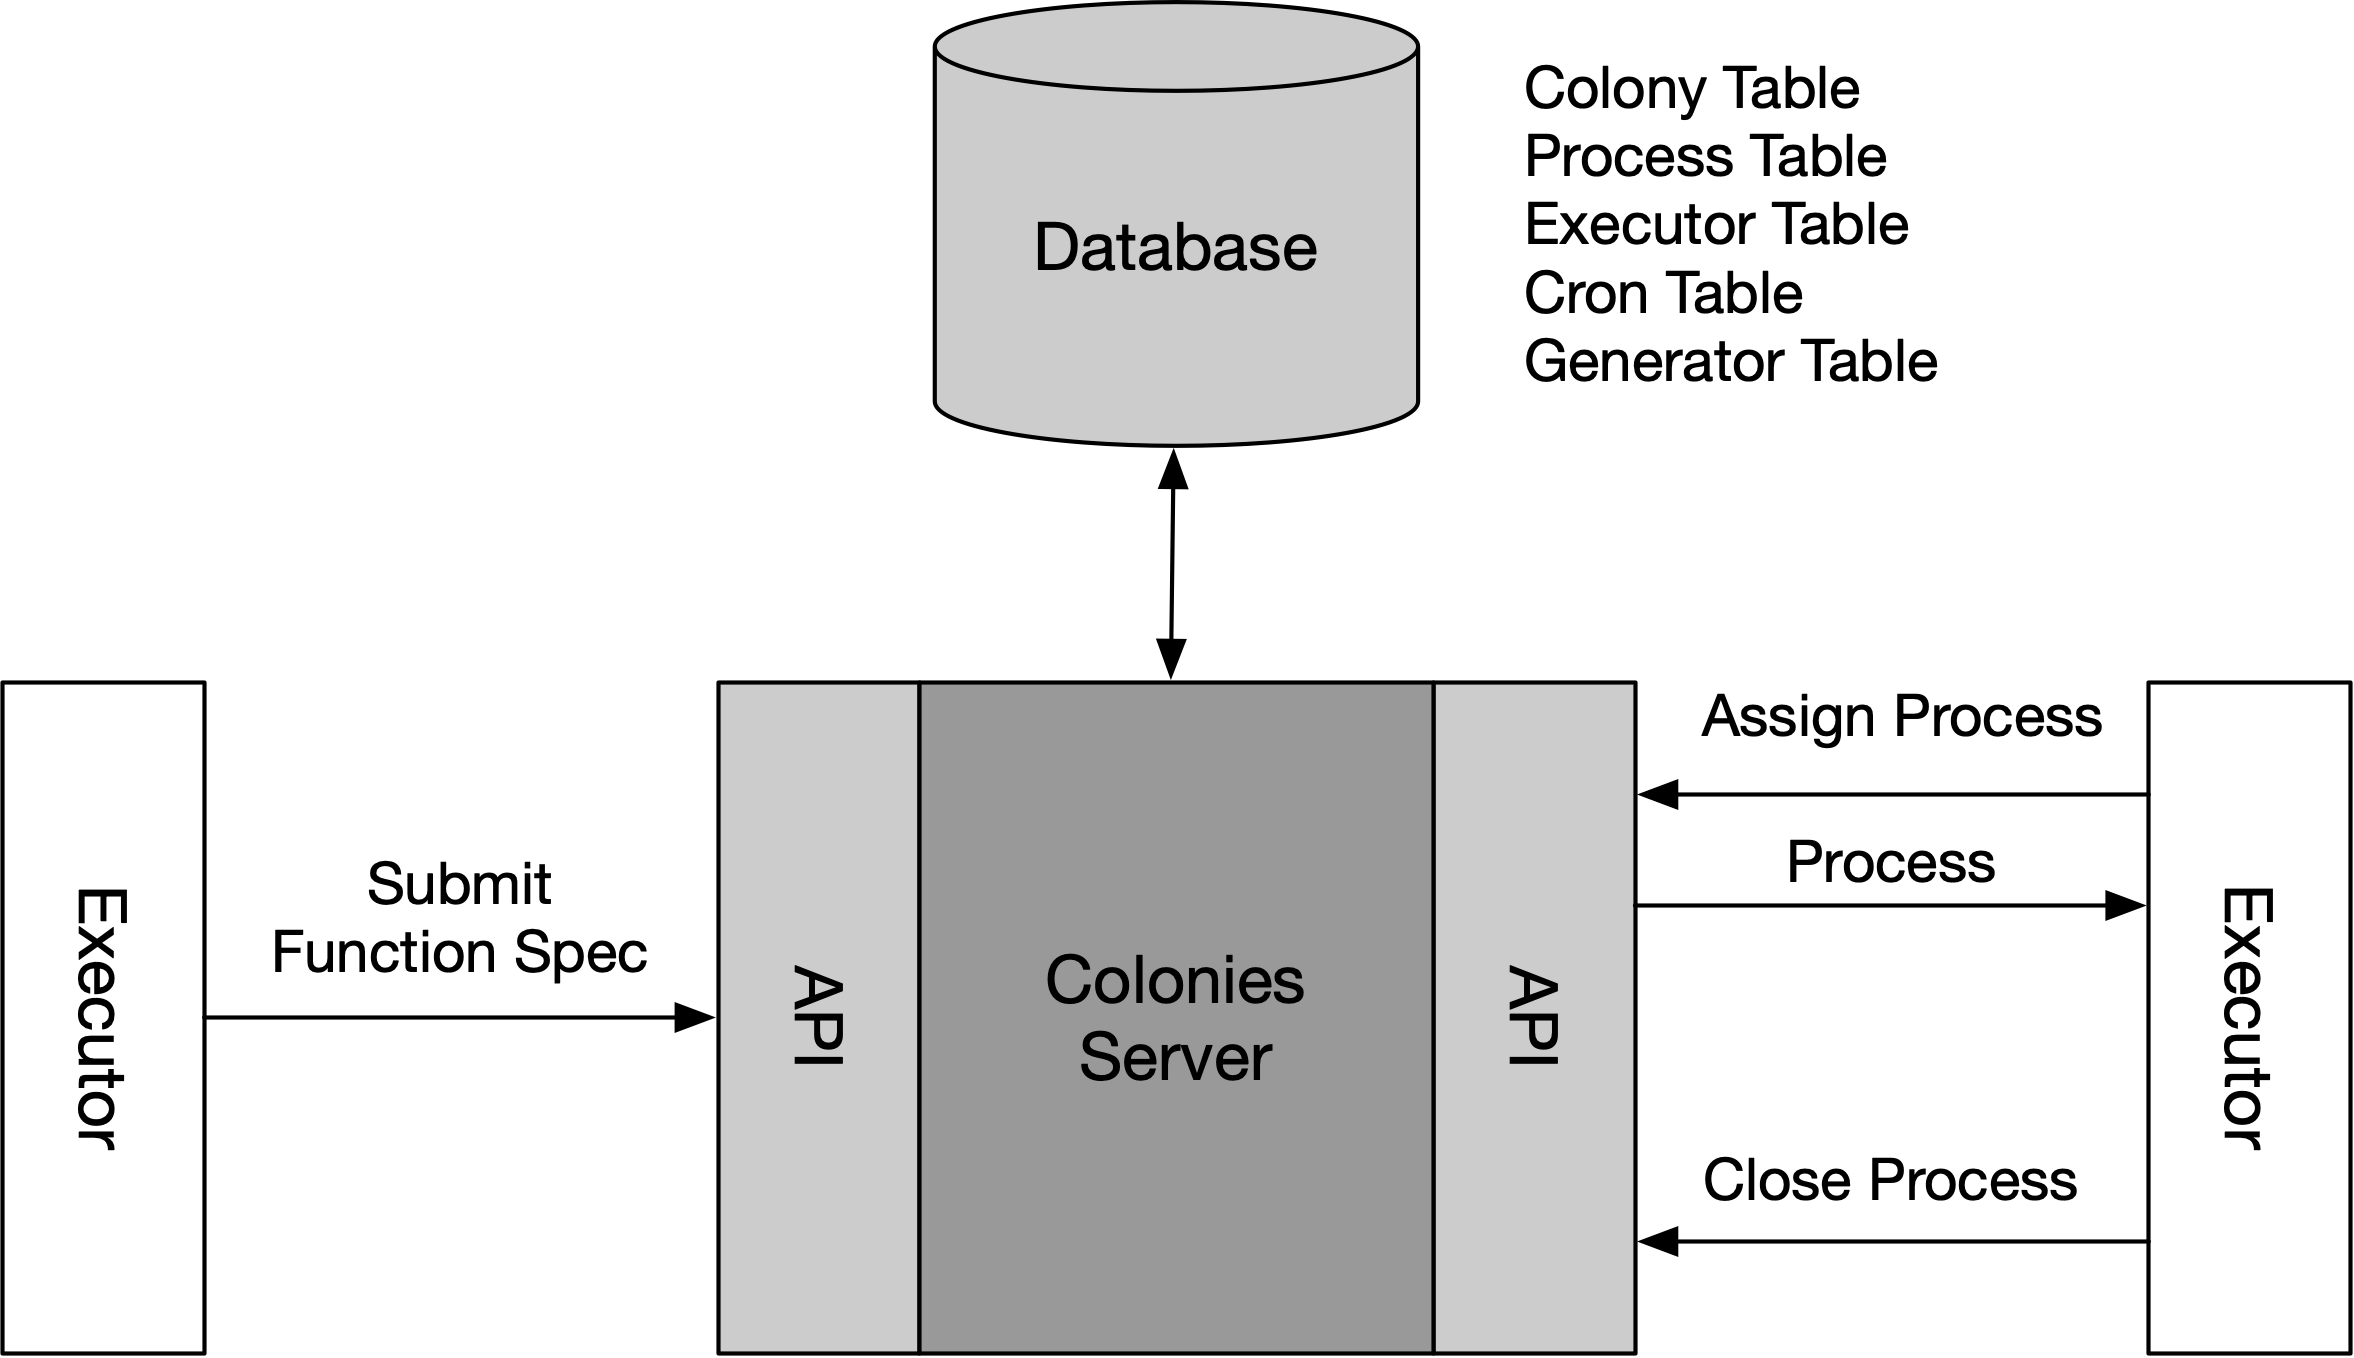
\includegraphics[scale=0.4]{arch.png}
	\caption{cron management}
	\label{fig:fig1}
\end{figure}

\begin{figure}[h]
	\centering
    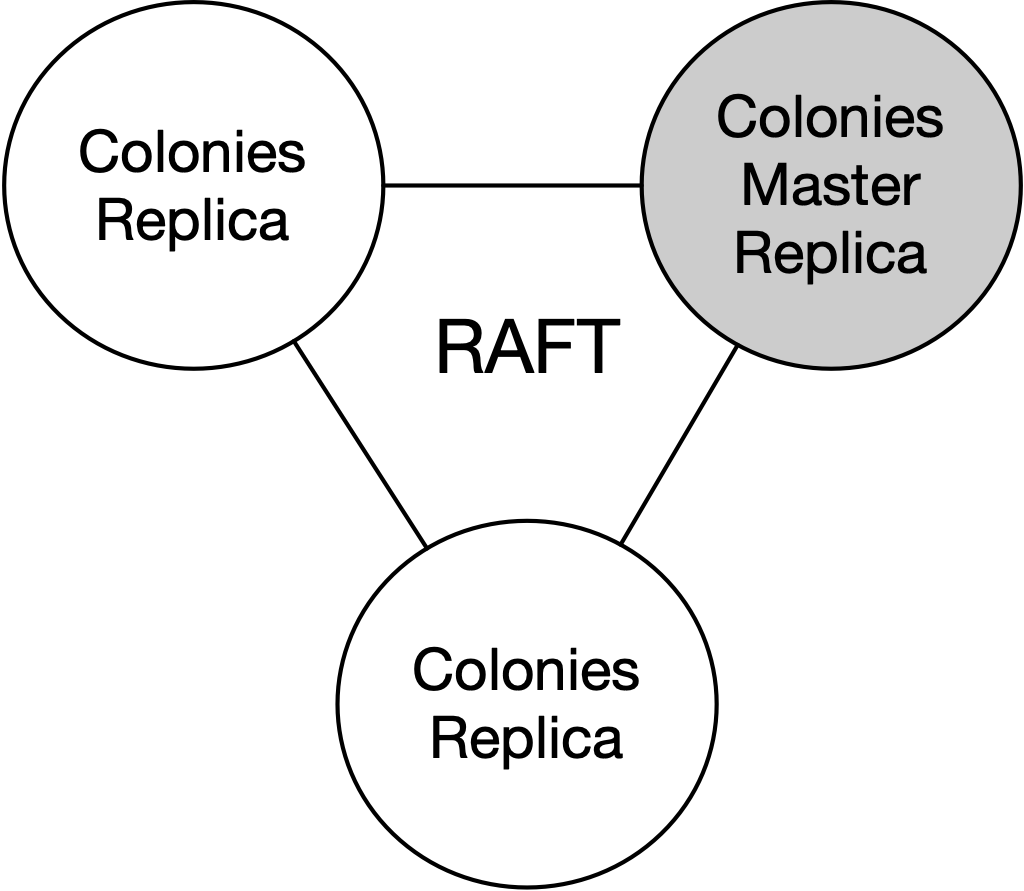
\includegraphics[scale=0.4]{raft.png}
	\caption{cron management}
	\label{fig:fig1}
\end{figure}

\subsubsection{Workflows}
TODO
\begin{figure}[h]
	\centering
    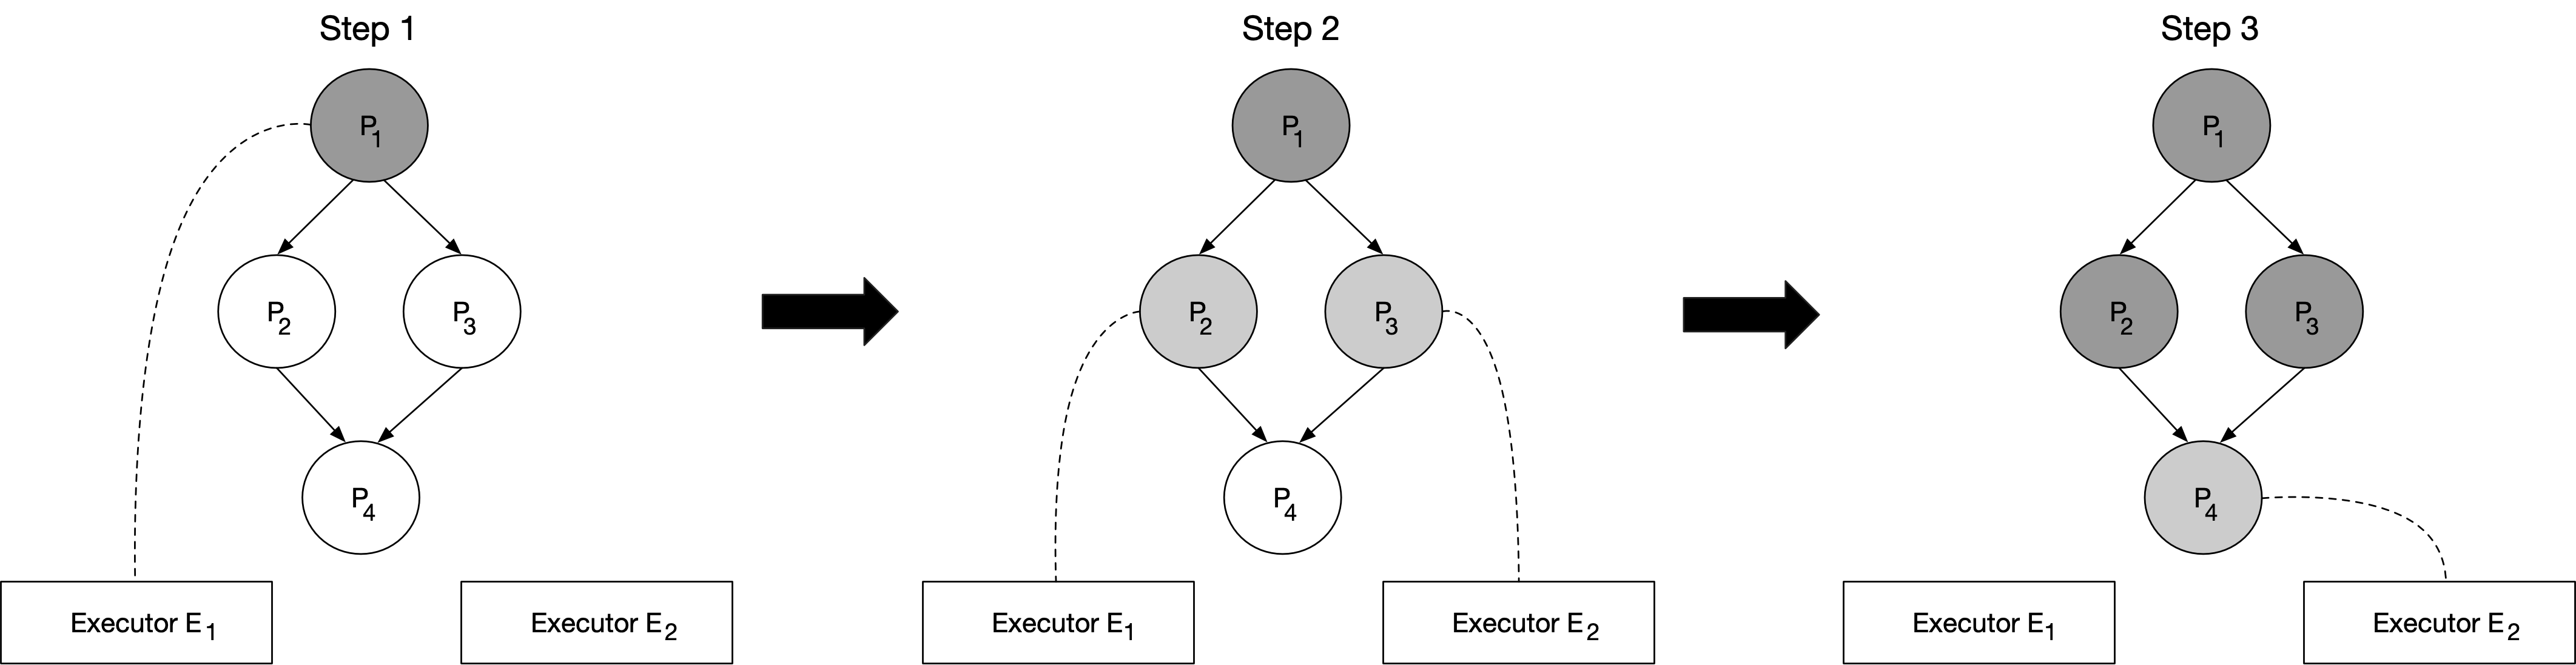
\includegraphics[scale=0.32]{workflow.png}
	\caption{cron management}
	\label{fig:fig1}
\end{figure}

\begin{table}[h]
	\caption{Function Specifications}
	\centering
	\begin{tabular}{llllll}
		\toprule
		\cmidrule(r){1-2}
        Function Spec & Function        & Executor Type & Priority & Max Exec Time & Max Retries \\
		\midrule
        $F_{1}$       & gen\_nums()     & Edge          & 1        & 200 s         & 5 \\
        $F_{2}$       & square()        & Cloud         & 1        & 200 s         & 5 \\
        $F_{3}$       & square()        & Cloud         & 1        & 200 s         & 5 \\
        $F_{4}$       & sum()           & Browser       & 1        & 200 s         & 5 \\
		\bottomrule
	\end{tabular}
	\label{tab:table}
\end{table}

\begin{table}[h]
	\caption{Snapshot of Process Table as in Step 2}
	\centering
	\begin{tabular}{llllll}
		\toprule
		\cmidrule(r){1-2}
        Process Id & Function Spec & Wait for Parents & Assigned Executor Id & State      & Priority Time \\
		\midrule
        $P_{1}$    & $F_{1}$       & $False$          & $E_{1}$              & Successful & 1679906715352024000 \\
        $P_{2}$    & $F_{2}$       & $False$          & $E_{1}$              & Running    & 1679906715353453000 \\
        $P_{3}$    & $F_{3}$       & $False$          & $E_{2}$              & Running    & 1679906715354286000 \\
        $P_{4}$    & $F_{4}$       & $True$           & -                    & Waiting    & 1679906715355188000 \\
		\bottomrule
	\end{tabular}
	\label{tab:table}
\end{table}

dt = -1000000000 * 60 * 60 * 24
process.PriorityTime = int64(process.FunctionSpec.Priority)*dt + submissionTime.UnixNano()


\begin{table}[h]
	\caption{Dependency Table}
	\centering
	\begin{tabular}{lll}
		\toprule
		\cmidrule(r){1-2}
        Process Id & Name       & Dependencies           \\
		\midrule
        $P_{1}$    & $Task_{1}$ & -                      \\
        $P_{2}$    & $Task_{2}$ & $Task_{1}$             \\
        $P_{3}$    & $Task_{3}$ & $Task_{1}$             \\
        $P_{4}$    & $Task_{4}$ & $Task_{2}$, $Task_{3}$ \\
		\bottomrule
	\end{tabular}
	\label{tab:table}
\end{table}
	
\begin{table}[h]
	\caption{Input/Output Table}
	\centering
	\begin{tabular}{lll}
		\toprule
		\cmidrule(r){1-2}
        Process Id & Input & Output \\
		\midrule
        $P_{1}$    & & [2,3] \\
        $P_{2}$    & 2 & 4 \\
        $P_{3}$    & 3 & 9 \\
        $P_{4}$    & [4,9] & 13 \\
		\bottomrule
	\end{tabular}
	\label{tab:table}
\end{table}

\subsubsection{Cron}
TODO
\begin{figure}[h]
	\centering
    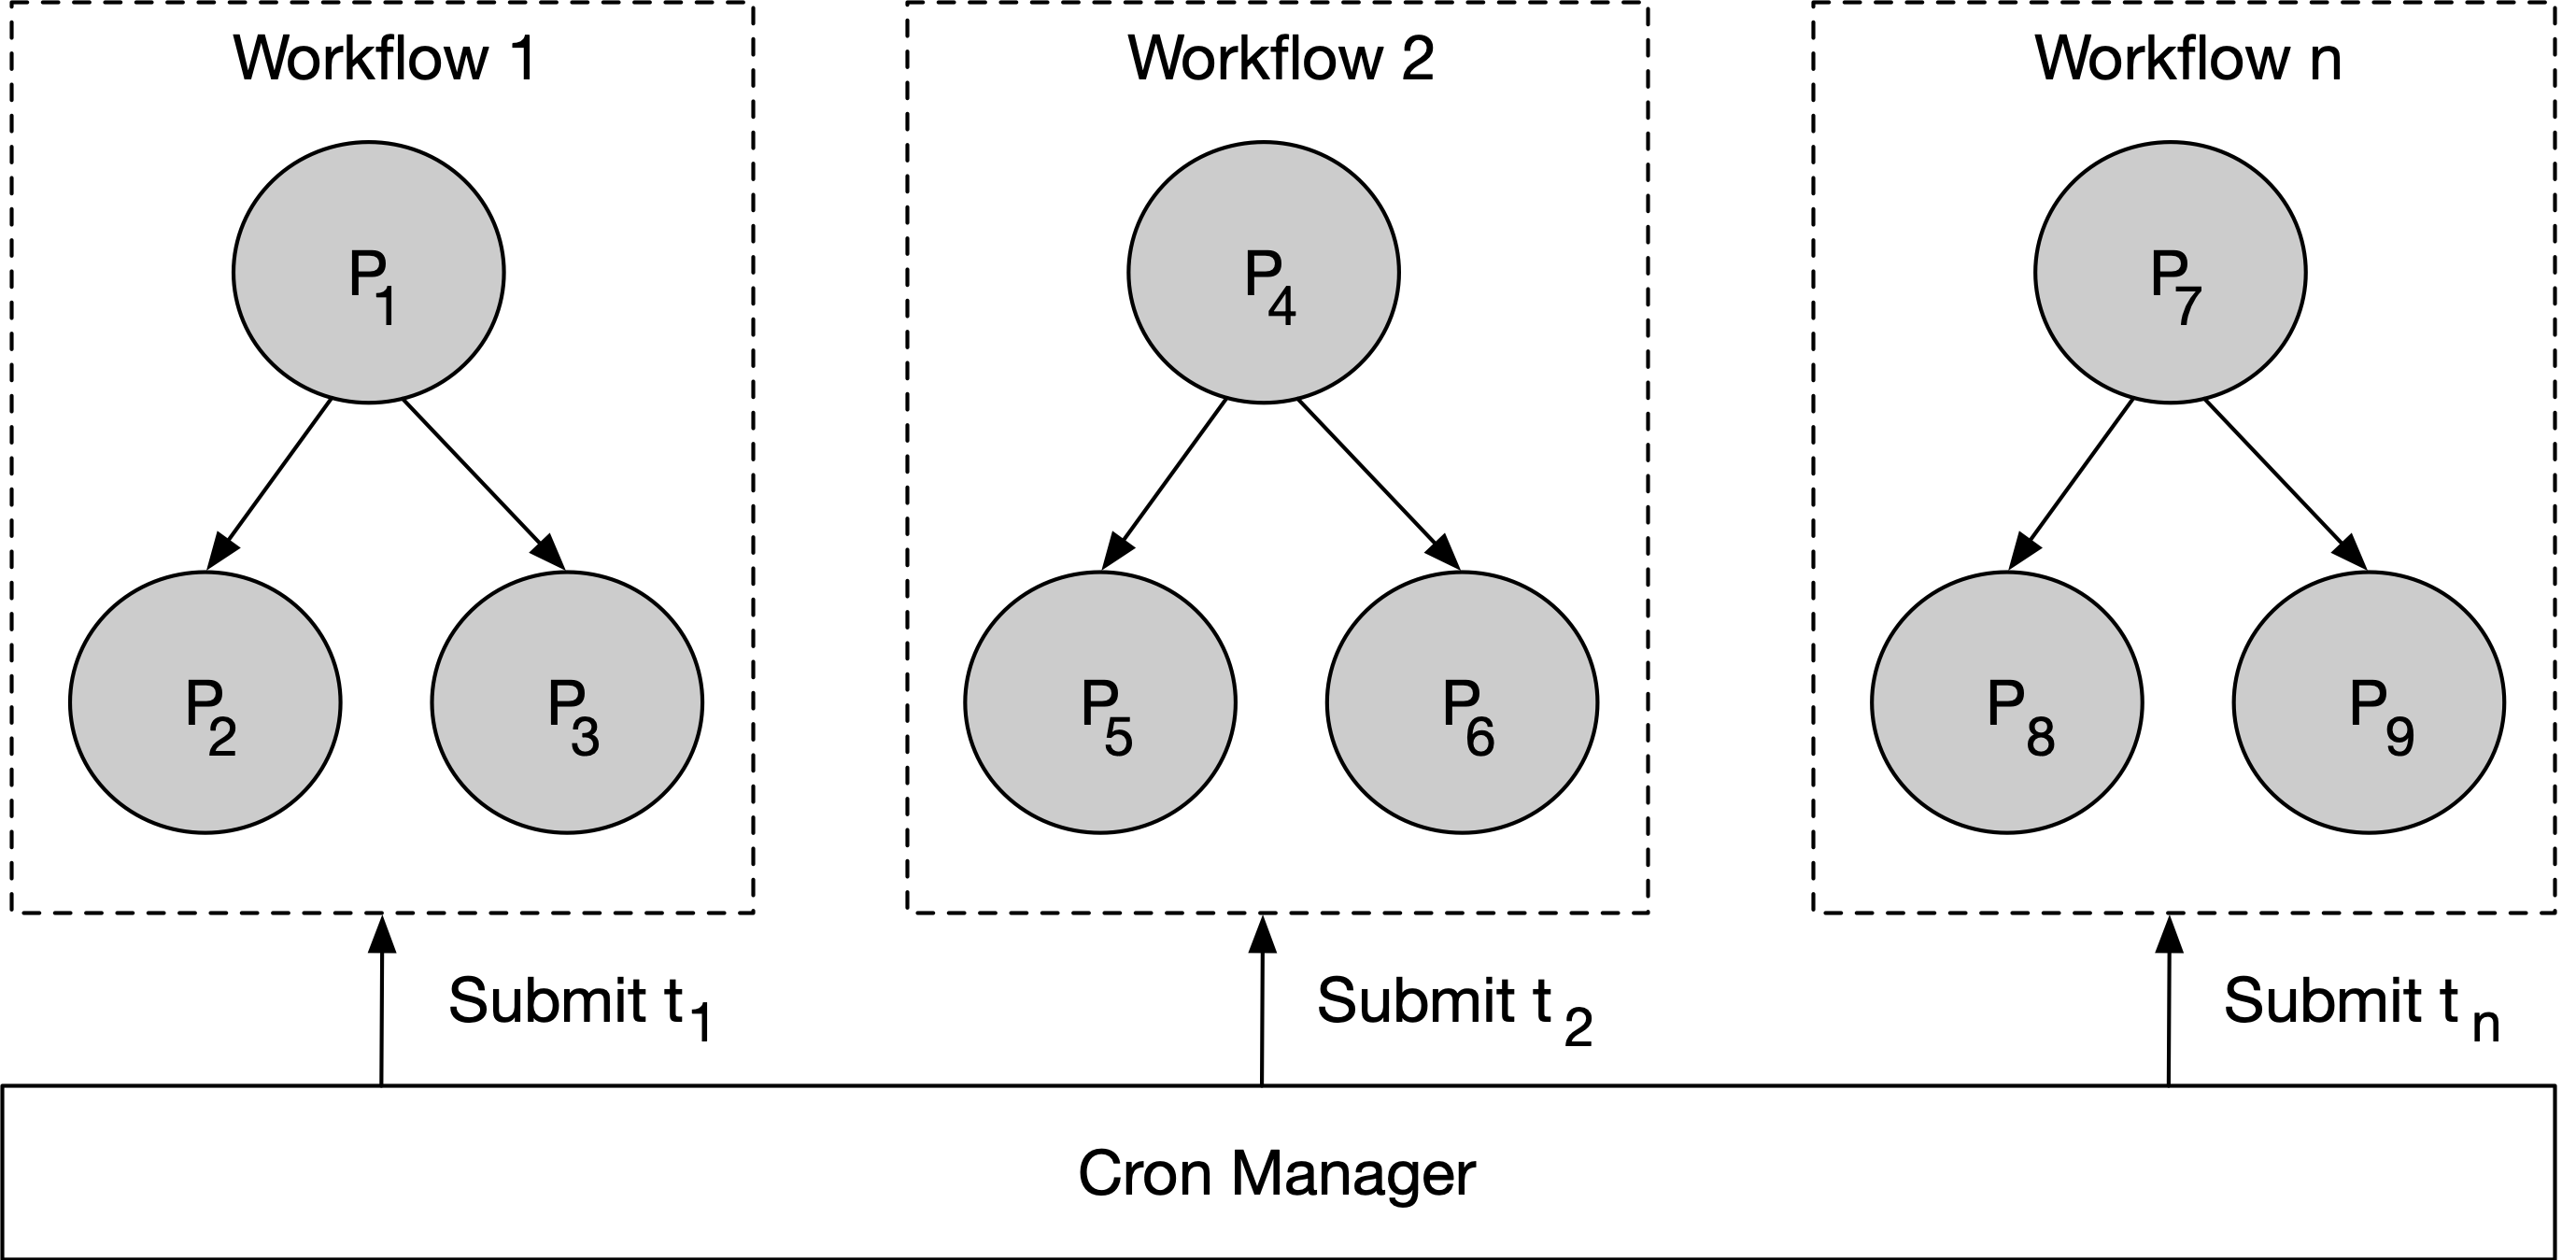
\includegraphics[scale=0.4]{cron.png}
	\caption{Sample figure caption.}
	\label{fig:fig1}
\end{figure}

\subsubsection{Generators}
TODO

\subsubsection{Zero-trust security}
TODO

\section{Evaluation}
\subsection{Implementation}
\begin{lstlisting}[language=c]
gen_nums = Function(gen_data, colonyid, executortype="edge")
square1 = Function(square, colonyid, executortype="cloud")
square2 = Function(square, colonyid, executortype="cloud")
sum = Function(square, colonyid, executortype="browser")

wf = ColoniesWorkflow("localhost", 50080, colonyid, executor_prvkey)
wf >> gennums
gennums >> square1
gennums >> square2
[square1, square2] >> sum
res = wf.execute()
\end{lstlisting}

\subsection{References}
TODO
\bibliographystyle{unsrtnat}
\bibliography{references}  %%% Uncomment this line and comment out the ``thebibliography'' section below to use the external .bib file (using bibtex) .


%%% Uncomment this section and comment out the \bibliography{references} line above to use inline references.
% \begin{thebibliography}{1}

% 	\bibitem{kour2014real}
% 	George Kour and Raid Saabne.
% 	\newblock Real-time segmentation of on-line handwritten arabic script.
% 	\newblock In {\em Frontiers in Handwriting Recognition (ICFHR), 2014 14th
% 			International Conference on}, pages 417--422. IEEE, 2014.

% 	\bibitem{kour2014fast}
% 	George Kour and Raid Saabne.
% 	\newblock Fast classification of handwritten on-line arabic characters.
% 	\newblock In {\em Soft Computing and Pattern Recognition (SoCPaR), 2014 6th
% 			International Conference of}, pages 312--318. IEEE, 2014.

% 	\bibitem{hadash2018estimate}
% 	Guy Hadash, Einat Kermany, Boaz Carmeli, Ofer Lavi, George Kour, and Alon
% 	Jacovi.
% 	\newblock Estimate and replace: A novel approach to integrating deep neural
% 	networks with existing applications.
% 	\newblock {\em arXiv preprint arXiv:1804.09028}, 2018.

% \end{thebibliography}

\end{document}
